\section{Attacking the Metering Model of EVM}
\label{sec:3:attack}
In light of the results we obtained in the previous sections, we hypothesise that it is possible to construct contracts which use a low amount of gas compared to the resources they use.

\subsection{Constructing Resource Exhaustion Attacks}
In particular, as we showed in \autoref{sec:3:case-studies}, the gas consumption is dominated by the storage allocated but is not as much affected by other resources such as the clock time. Therefore, we decide to use the clock time as a target resource and look for contracts which minimise the throughput in terms of gas per second. We can formulate this as a search problem.

\point{Problem formulation}
We want to find a program which has the minimum possible throughput, where we define the throughput to be the amount of gas processed per second.
Let $\mathbb{I}$ be the set of EVM instructions and $P$ be the set of EVM programs. A program $p\in P$ is a sequence of instructions $I_1,\cdots,I_n$ where all $I_i \in \mathbb{I}$. Let $t : P \rightarrow \mathbb{R}$ be a function which takes a program as an input and outputs its execution time and $g : P \rightarrow \mathbb{N}$ be a function which takes a program as input and outputs its gas cost. We define our function to minimise $f: P \rightarrow \mathbb{R},~f(p) = g(p) / t(p)$. Our goal is to find the program $p_{\text{slowest}}$ such that

\begin{equation}
  \label{eq:objective}
  p_{\text{slowest}} = \argmin_{p\in P} (f(p))
\end{equation}

The search space for a program of size $n$ is $|\mathbb{I}|^n$. Given $|\mathbb{I}| \approx 100$, the search space is clearly too large to be explored entirely for any non-trivial program. Therefore, we cannot simply go over the space of possible programs and instead need to approximate the solution.

Although our problem resembles other program synthesis tasks~\cite{gulwani2017program}, there is a notable difference. Program synthesis usually focuses on generating ``meaningful'' programs, either from specifications or examples. These tasks often do not have well-defined metrics allowing optimisation techniques (the genetic algorithm in our work). The task we solve is different because we need to define ``valid'' but not ``meaningful'' programs and optimise for a well-defined metric: gas throughput.

\point{Search strategy}
With the problem formulated as a search problem, we now present our search strategy. We decide to design the search as a genetic algorithm~\cite{whitley1994genetic}. The reasons for this choice are as follows:

\begin{itemize}
  \item we have a well-defined fitness function $f$
  \item we have promising initialisation values, which we will discuss below
  \item programs being a sequence of instructions, cross-over and mutations can be designed efficiently
  \item programs generated need to be syntactically correct but do not need to be semantically meaningful, making the cross-over and mutations more straightforward to design
\end{itemize}
%
We will now discuss in detail how we design the initialisation, cross-over and mutations of our genetic algorithm.

\point{Program construction}
Although our programs do not need to be semantically meaningful, they need to be executed successfully on the EVM, which means that they must fulfil some conditions. First, an instruction should never try to consume more values than the current number of elements on the stack. Second, instructions should not try to access random parts of the EVM memory, otherwise, the program could run out of gas straight away. Indeed, when an instruction reads or writes to a place in memory, the memory is ``allocated'' up to this position and a fee is taken for each allocated memory word. This means that if \lstinline{MLOAD} would be called with $2^{100}$ as an argument, it would result in the cost of allocating $2^{100}$ words in memory, which would result in an out-of-gas exception.

  Another potential issue would be to run into an infinite loop. However, we decide to explicitly exclude loops from our program generation algorithm for the following reason: adding loops is unlikely to make the generated programs slower. Indeed, if a piece of code is slow enough, our genetic algorithm will tend to repeat it. The loop version could be faster if a value is already cached but have no reason to be slower.

  We design the program construction so that all created programs will never fail because of either of the previous reasons. We first want to ensure that there are always enough elements on the stack to be able to execute an instruction. The instructions requiring the least number of elements on the stack are instructions such as \lstinline{PUSH} or \lstinline{BALANCE} which do not require any element, and the element requiring the most number of elements on the stack is \lstinline{SWAP16} which requires $17$ elements to be on the stack.
  We define the functions function $a : \mathbb{I} \rightarrow \mathbb{N}$ which returns the number of arguments consumed from the stack and $r : \mathbb{I} \rightarrow \mathbb{N}$ which returns the number of elements returned on the stack for an instruction $I$. We generate 18 sets of instructions using \autoref{eq:instr-args}.

  \begin{equation}
    \label{eq:instr-args}
    \forall n \in [0, 17],~ \mathbb{I}_n = \{I~|~I\in \mathbb{I} \land a(I) \leq n\}
  \end{equation}

  For example, the set $\mathbb{I}_3$ is composed of all the instructions which require $3$ or fewer items on the stack.
  We will use these sets in \autoref{alg:construct-program} to construct the initial programs but before, we need to define the functions we use to control memory access. For this purpose, we define two functions to handle these. First, $uses\_memory : \mathbb{I} \rightarrow \{0, 1\}$ returns $1$ only if the given instruction accesses memory in some way. Then, $prepare\_stack: \mathbb{P}\times\mathbb{I}\rightarrow \mathbb{P}$ takes a program and an instruction and ensures that all the arguments of the instruction which influence which part of memory is accessed are below a relatively low value, that we arbitrarily set to $255$. To ensure this, $prepare\_stack$ adds \lstinline{POP} instruction for all arguments of $I$ and adds the same number of \lstinline{PUSH1} instructions with a random value below the desired value. For example, in the case of \lstinline{MLOAD}, a \lstinline{POP} followed by a \lstinline{PUSH1} would be generated.

  Using the sets $\mathbb{I}_n$, the $uses\_memory$ and $prepare\_stack$ functions, we use \autoref{alg:construct-program} to generate the program. We assume that the $biased\_sample$ function returns a random element from the given set and will discuss how we instantiate it in the next section.

  \begin{algorithm}
    \begin{algorithmic}
      \Function{GenerateProgram}{$size$}
      \State $P \gets (~)$\Comment{Initial empty program}
      \State $s\gets 0$\Comment{Stack size}
      \For{$1$ to $size$}
      \State $I \gets biased\_sample(\mathbb{I}_s$)
        \If{$uses\_memory(I)$}
        \State $P \gets prepare\_stack(P, I)$
        \EndIf
        \State $P \gets P \cdot (~I~)$\Comment{Append $I$ to $P$}
        \State $s \gets s + (r(I) - a(I))$
        \EndFor
        \State \textbf{return} $P$
      \EndFunction
    \end{algorithmic}
    \caption{Initial program construction}
    \label{alg:construct-program}
  \end{algorithm}


  \point{Initialisation}
  As the search space is very large, it is important to start with good initial values so that the genetic algorithm can search for promising solutions. For this purpose, we use the result of the results we presented in \autoref{sec:3:case-studies}, in particular, we use the throughput measured for each instruction. We define a function $throughput : \mathbb{I} \rightarrow \mathbb{R}$ which returns the measured throughput of a single instruction. When randomly choosing the instructions with $biased\_sample$, we want to have a higher probability of picking an instruction with a low throughput but want to keep a high enough probability of picking a higher throughput instruction to make sure that these are not all discarded before the search begins. We define the weight of each instruction and then its probability with \autoref{eq:initial-weight} and \autoref{eq:initial-prob}.

  \begin{align}
    \label{eq:initial-weight}
    W(I\in \mathbb{I})   & = \log\left(1 + \frac{1}{throughput(I)}\right) \\
    \label{eq:initial-prob}
    P(I\in \mathbb{I}_n) & = \frac{W(I)}{\sum_{I'\in \mathbb{I}_n}W(I')}
  \end{align}
  %
  Given that the throughput can have order-of-magnitude differences among instructions, the $\log$ in \autoref{eq:initial-weight} is used to avoid assigning a probability too close to~$0$ to an instruction.

  \point{Cross-over}
  We now want to define a cross-over function over our search space, a function which takes as input two programs and returns two programs, i.e. $cross\_over : \mathbb{P} \times \mathbb{P} \rightarrow \mathbb{P} \times \mathbb{P}$, where the output programs are combined from the input programs. To avoid enlarging the search space with invalid programs, we want to perform a cross-over such that the two output programs are valid by construction.
  During program creation, we must ensure that each instruction of the output program will always have enough elements on the stack and that it will not try to read or write at random memory locations.

  For the memory issue, we simply avoid modifying the program before an instruction manipulating memory or one of the \lstinline{POP} or \lstinline{PUSH1} added in the program construction phase. For the second issue, we make sure to always split the two programs at positions where they have the same number of elements on the stack.

  We show how we perform the cross-over in \autoref{alg:cross-over}. In the \textproc{CreateStackSizeIndex} function, we create a mapping from a stack size to a set of program counters where the stack has this size. In the \textproc{CrossOver} function, we first create this mapping for both programs and randomly choose a stack size to split the program. We then randomly choose a location from each program with the selected stack size. Note that here, $sample$ assigns the same probability to all elements in the set. Finally, we split each program in two at the chosen position, and cross the programs together.

  \begin{algorithm}
    \begin{algorithmic}
      \Function{CreateStackSizeMapping}{$P$}
      \State $S \gets $ \text{empty mapping}
      \State $pc \gets 0$
      \State $s \gets 0$
      \For{$I~\text{in}~P$}
      \If{$s\notin S$}
      \State $S[s] \gets \{\}$
      \EndIf
      \State $S[s] \gets S[s] \cup \{pc\}$
      \State $s \gets s + (r(I) - a(I))$
      \State $pc \gets pc + 1$
      \EndFor
      \State \textbf{return} $S$
      \EndFunction

      \Function{CrossOver}{$P_1, P_2$}
      \State $S_1 \gets$~\Call{CreateStackSizeMapping}{$P_1$}
      \State $S_2 \gets$~\Call{CreateStackSizeMapping}{$P_2$}
      \State $S \gets S_1 \cap S_2$\Comment{Intersection on keys}
      \State $s \gets sample(S)$
      \State $i_1 \gets sample(S_1[s])$
      \State $i_2 \gets sample(S_2[s])$
      \State $P_{11}, P_{12} \gets split\_at(P_1, i_1)$
      \State $P_{21}, P_{22} \gets split\_at(P_2, i_2)$
      \State $P_1' \gets P_{11}\cdot P_{22}$\Comment{Concatenate}
      \State $P_2' \gets P_{21}\cdot P_{12}$
      \State \textbf{return} $P_1',~P_2'$
      \EndFunction
    \end{algorithmic}
    \caption{Cross-over function}
    \label{alg:cross-over}
  \end{algorithm}

  \point{Mutation}
  We use a straightforward mutation operator. We randomly choose an instruction $I$ in the program,  where $I$ is not one of the \lstinline{POP} or \lstinline{PUSH1} instructions added to handle memory issues previously discussed. We generate a set $M_I$ of replacement candidate instructions defined as follows.
  \begin{equation}
    \label{ref:mutation-set}
    M_I = \{ I'~|~I'\in \mathbb{I}_{a(I)}\land r(I') = r(I) \}
  \end{equation}

  In other words, the replacement must require at most the same number of elements on the stack and put back the same number as the replaced instruction. Then, we replace the instruction $I$ with $I'$, which we randomly sample from $M_I$. If $I$ had \lstinline{POP} or \lstinline{PUSH1} associated with it to control memory, we remove them from the program. Finally, if $I^\prime$ uses memory, we add the necessary instructions before it.

  \subsection{Effectiveness of Attacks with Synthetic Contracts}
  \begin{figure}[tb]
    \centering
    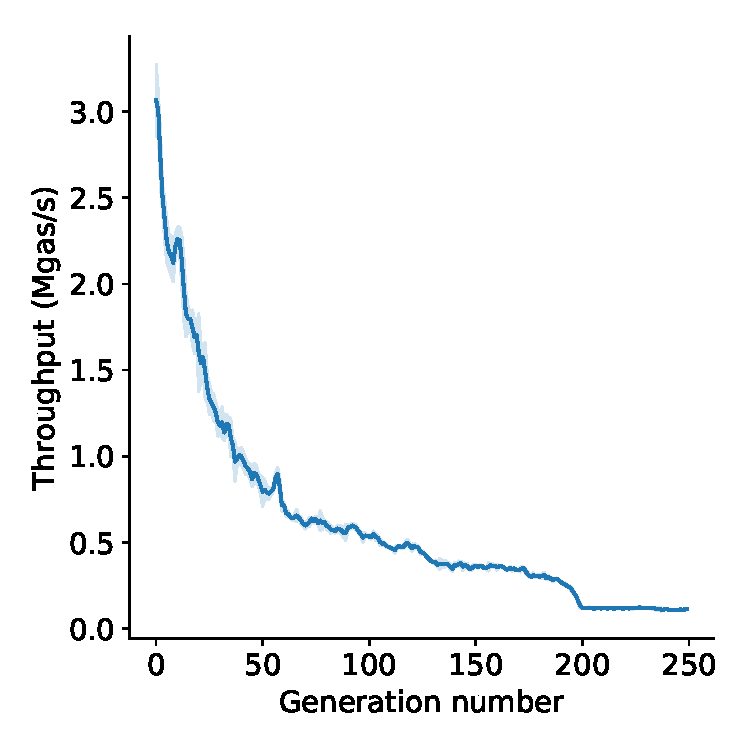
\includegraphics[width=.8\columnwidth]{./3-vm-security/figures/ga-contract-gas-results.pdf}
    \caption[Evolution of the throughput as a function of the number of generations]{Evolution of the average contract throughput as a function of the number of generations.}
    \label{fig:throughput-evolution}
  \end{figure}

  \begin{figure}[tb]
    \centering
    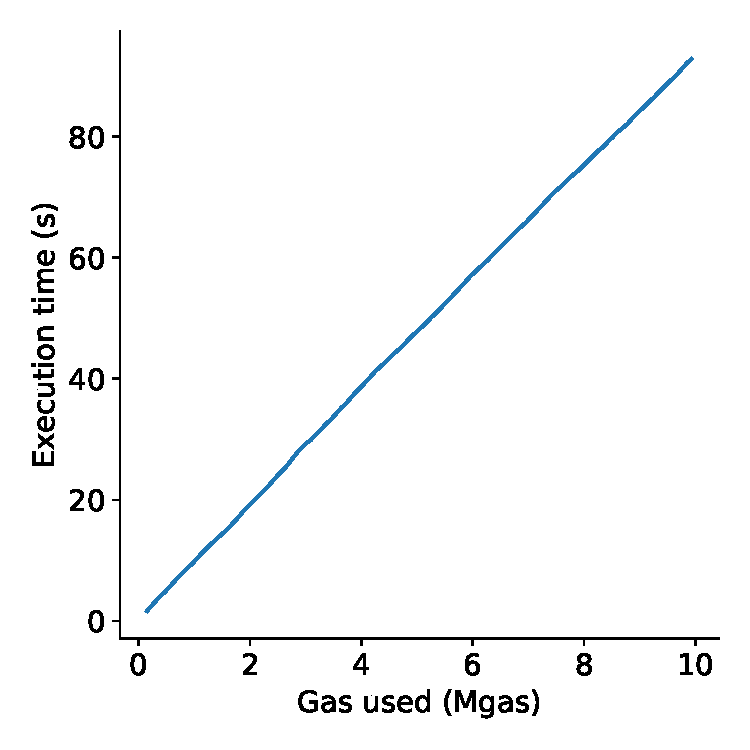
\includegraphics[width=.7\columnwidth]{./3-vm-security/figures/block-execution-time.pdf}
    \caption[Execution time as a function of the gas used by contracts within a block]{Execution time as a function of the total amount of gas used by contracts within a block.}
    \label{fig:block-exec-speed}
  \end{figure}

  We want to measure the effectiveness of our approach to produce Resource Exhaustion Attacks. To do so, we want to generate contracts and benchmark them while mimicking the behaviour of a regular full validating node as much as possible. To do so, we execute all the programs produced within every generation of our genetic algorithm, as if they were part of a single block. We use the following steps to run our genetic algorithm.

  \begin{enumerate}
    \item Clear the page cache;
    \item Warm up caches by generating and executing randomly-generated contracts
    \item Generate the initial set of programs;
    \item Run the genetic algorithm for~$n$ generation.
  \end{enumerate}
  %
  An important point here is that when running the genetic algorithm, we only want to execute each program once, otherwise every IO access will already be cached and it will invalidate the results, as this is not what would happen when a regular validating node executes contracts. However, we of course do want to execute the measurements multiple times to be able to measure the execution time standard deviation. To work around these two requirements, we save all the programs generated while we run the experiment.
  Once the experiment has finished, we re-run all the programs in the same order. We combine these results to compute the mean and standard deviation of the execution time.

  We note that generating a new generation takes on average less than~\empirical{1} second but the time-consuming part of our algorithm is to compute the throughput of the generated programs. Indeed, we need to wait for the EVM to run the program, which can, as we show in this section, take more than~\empirical{90} seconds for a single generation. Furthermore, parallelising this task could bias our measurements, which forces the algorithm to perform the evaluation serially.

\begin{lstlisting}[escapeinside={<@}{@>},language=esm,basicstyle=\small\ttfamily,float=tp,floatplacement=tbp,caption=Bytecode snippet generated by our genetic algorithm. Instructions in bold involve some sort of IO operations.,label=list:generated-code]
PUSH9 0x57c2b11309b96b4c59
<@\textbf{BLOCKHASH}@>
<@\textbf{SLOAD}@>
CALLDATALOAD
PUSH7 0x25dfb360fa775a@
<@\textbf{BALANCE}@>
MSTORE8
PUSH10 0x49f8c33edeea6ac2fe8a
PUSH14 0x1d18e6ece8b0cdbea6eb485ab61a
<@\textbf{BALANCE}@>
POP      ; prepare call to CALLDATACOPY
POP
POP
PUSH1 0xf7
PUSH1 0xf7
PUSH1 0xf7
<@\textbf{CALLDATACOPY}@>
PUSH7 0x421437ba67fe0e
ADDRESS
<@\textbf{BLOCKHASH}@>
\end{lstlisting}

  \point{Generated bytecode}
  Before discussing the results further, we show a small snippet of bytecode generated by our genetic algorithm in \autoref{list:generated-code}. We highlight the instructions which involve IO operations in bold and show the instructions whose sole purpose is to keep the stack consistent in a smaller font. We can see that there is a large number of IO-related instructions, in particular, \lstinline{BLOCKHASH} and \lstinline{BALANCE} show up multiple times. Although the fee of \lstinline{BALANCE} has been revised from~20 to~400 in EIP-150, this suggests that the instruction is still under-priced. In the snippet, we also see that the stack is cleared and replaced with small values before calling \lstinline{CALLDATACOPY}. This corresponds to the $prepare\_stack$ function described in the program construction section: to avoid \lstinline{CALLDATACOPY} reading very far away in memory, which would make the program run out of gas, the arguments are replaced with small values. We note that our algorithm can generate programs of arbitrary length but in our experiments, we set it to create programs of around~\empirical{4,000} instructions which consume between~\empirical{100,000} and \empirical{150,000} gas.

  \point{Generating low-throughput contracts}
  We show how the throughput of the lowest-performing contract evolved with the number of generations in \autoref{fig:throughput-evolution}. The line represents the mean of the measurements and the band represents the standard deviation of the measurements. The measurements are run~\empirical{3} times.
  Except for one point in the first measurements, overall the standard deviation remains relatively low.

  We can see that during the first generations, the throughput is around~\empirical{1.25M} gas per second, which is already fairly low given that the average throughput for a transaction on the same machine is around~\empirical{20M} gas per second. This shows that our initialisation is effective. The throughput decreases very quickly in the first few generations, and then steadily decreases down to around~\empirical{110K} gas per second, which is more than~\empirical{180} slower than the average transaction. After about~\empirical{200} generations, the throughput plateaus.

  \point{Exploring the minimum}
  The minimum in our experiments is attained at generation~\empirical{243}. At this point, the block uses in total approximately~\empirical{9.9M} gas and takes around~\empirical{93~seconds} to execute, or throughput of about~\empirical{107,000} gas per second. We show in \autoref{fig:block-exec-speed} how the execution time increases with the amount of gas consumed within the block.
  It is important to note that the execution time increases perfectly linearly with the gas used, which means that all transactions in the block have almost the same throughput. This implies that an attacker could easily tune the time he wants to delay the nodes depending on his budget. If a block full of malicious transactions were to be processed, given that an Ethereum block is produced roughly every 13 seconds,~\empirical{7} new blocks would have been created by the time the node finishes validating the malicious one.

  \begin{table}
    \centering
    \setlength{\tabcolsep}{3pt}
    \caption[Evaluation of different Ethereum clients]{Evaluation of different clients when executing 10M gas worth of malicious transactions. What is presented is the mean across \empirical{three} measurements~$\pm$ standard deviation. All the measurements are performed on our GCP except the ``metal'' which is done on our bare-metal server.}
    \label{tab:clients-evaluation}
    \begin{tabular}{l r r r}
      \toprule
      \multirow{2}{*}{\textbf{Client}} & \textbf{Throughput}             & \textbf{Time}   & \textbf{IO load} \\
                                       & Gas/s                           & second          & MB/s             \\
      \midrule
      Aleth                            & $107,349\pm 606.6$              & $93.6\pm 0.53$  & $9.12\pm 4.70$   \\
      Parity                           & $210,746\pm 7,672$              & $47.1\pm 1.61$  & $10.0\pm 1.36$   \\
      Parity (\small{metal})           & $542,702\pm 9,487$              & $18.2\pm 0.23$  & $17.2\pm 1.97$   \\
      Geth                             & $131,053\pm 4,207$              & $75.6\pm 2.42$  & $6.57\pm 4.13$   \\
      Geth (\small{fixed})             & $3,021,038 \pm 4.67\mathrm{e}5$ & $3.33 \pm 0.56$ & $0.72\pm 0.11$   \\
      \bottomrule
    \end{tabular}
  \end{table}

  \subsection{Evaluation on Other Ethereum Clients}
  We used aleth~\cite{aleth} to run our genetic algorithm and find low-throughput contracts. In this section, we show that the contracts crafted using our algorithm are also effective on the two most popular Ethereum clients: geth~(v1.9.6)~\cite{geth} and Parity Ethereum~(v2.5.9)~\cite{parity-ethereum}. We also show that the fix released in geth following discussions with the development team successfully resolves the issue. our attack is mainly efficient on less powerful hardware, we include the measurements of Parity on a more powerful bare-metal machine with 4 cores (8 threads) at 2.7GHZ, 32GB of RAM and an SSD with 540MB/s throughput.
  %
  To benchmark the clients, we use the following procedure and repeat the measurements \empirical{three} times for each client.

  \begin{enumerate}
    \item Synchronise the client to test;
    \item Start the client in a private network so that it does not execute anything else but our contracts;
    \item Execute transactions on the client using the \lstinline{eth_call} RPC endpoint;
          \begin{enumerate}
            \item Send transactions to warm up the client
            \item Send enough malicious transactions to consume 10M gas
          \end{enumerate}
    \item Measure the gas, time, IO, CPU and memory used during the execution of the malicious transactions.
  \end{enumerate}
  %
  We report our results in~\autoref{tab:clients-evaluation}. Although we measured CPU, memory, and IO usage, most of the used time was related to IO operations and there was no significant increase in either CPU or memory usage during the attack. Therefore, we only report the IO measurements collected during the attack. We express the IO load in terms of MB/s, which we collect using Linux's \texttt{iotop} utility.

  Before geth's fix, geth takes more than~$75$ seconds to execute~10M gas worth of malicious transactions. Parity Ethereum is the least vulnerable to our attack, but still takes on average about~$47$ seconds. Parity has on average a higher, but more constant IO load than geth.
  Large increases in the IO load tend to increase the IO wait time, which could explain why geth is vastly slower than Parity. Aleth is the slowest of the three clients. There could be two reasons for this: first, our algorithm is optimised on aleth, which makes it more likely to slow it down, second, aleth is less actively developed than the other two clients and might lack some optimisations.

  The results of running Parity on a more powerful bare-metal server show that even such machines are relatively vulnerable to our attack. Indeed, Parity, which was the fastest of the three clients, still took more than~\empirical{18} seconds to execute the transactions. An important point to notice is that the IO throughput is considerably higher on our bare-metal server, which is most likely one of the main reasons for the speedup.

  Finally, we ran our attack on an improved version of geth, which the Ethereum developers pointed us to as a result of our interactions with them. This version includes several optimisations to improve the storage access speed. We can see that these improvements drastically reduced the IO load of the client. With these improvements, geth executes the transactions more than 20 times faster, making the execution speed fast enough to counter such an attack.
  Our interaction with geth developers shows the effectiveness of responsible vulnerability disclosure, as discussed in \autoref{sec:3:responsible}.

  \subsection{REA as a Form of DoS}
  Malicious contracts crafted using our algorithm could easily be used to perform a DoS attacks on Ethereum. In this section, we will describe the threat model of such an attack, including the implications and feasibility of the attack.

  \point{Attack implications}
  As described in \autoref{sec:3:background}, there have already been several instances of DoS attacks against Ethereum~\cite{transaction-spam-attack,suicide-attack}.
  There are several consequences to such attacks.
  The most direct one is a high increase in the block production time~\cite{average-block-time}, which in the worst cases more than doubled, significantly decreasing the total throughput of the network.
  This decrease comes not only from miners who might take more time to validate blocks but also from full nodes who are supposed to relay validated blocks and might take vastly longer to do so.
  A further indirect consequence of such attacks is the loss of trust in the system, which can lead to a decrease in the price of Ethereum, at least for a short period of time~\cite{Chen2017Metering}.

  \point{Probable attacker}
  Although instances of irrational behaviours with likely no profit to the attacker have been seen on Ethereum~\cite{Breidenbach}, we assume that the attacker is rational and wants to profit from such an attack. In this context, there are several ways in which such an attack could be performed.

  First, this attack could be beneficial to miners. A miner could use these malicious transactions to perform a sort of selfish-mining~\cite{eyal2014majority}.
  Indeed, if the miner chooses to include a small number of malicious transactions in the blocks he mines, the propagation time per block is likely to increase and give the miner a head start on mining the next block.
  Given that the block arrival time in Ethereum is around 12 seconds, gaining a couple of seconds can be financially interesting for a miner. Furthermore, the only cost for a miner would be the opportunity cost of not including other transactions in the block, as he could include malicious transactions with a gas price of 0.

  Another potential motivation for an attack could be to try to reduce the price of the ETH token and the trust in the Ethereum ecosystem. An attacker wanting to make a one-shot profit could spend some amount of money into performing such a DoS attack while taking a short position on ETH, waiting for the price to go down. Other blockchains competing with Ethereum could also potentially use such tactics to try to discredit the reliability of Ethereum.

  \point{Attack feasibility}
  To reason about the feasibility of this attack, we assume that given the same gas price, a malicious transaction has the same chance of being included in a block as any other transaction. We use the time we obtained in our experiments with geth, as it is the Ethereum client with the largest usage share~\cite{ehternodes}.

  To find a reasonable gas price, we analyse the gas price of all transactions and blocks from~\empirical{October 1, 2019 (block 8,653,171)} to \empirical{December 31, 2019 (block 9,193,265)}. We find that the median value of the minimum gas price in a block is around~\empirical{1.1Gwei} and that the average gas price is around~\empirical{10Gwei} with a standard deviation of~\empirical{11Gwei}. These values are in agreement with some other source of gas computation~\cite{eth-gas-station}. Finally, we find that at least \empirical{2 million} gas worth of transactions are included for less than~\empirical{3Gwei} in about~\empirical{90\%} of the blocks, and choose this value as the gas price to compute the cost of an attack.

  Given that our malicious transactions have a throughput of about~131,000 gas per second, using a price of~\empirical{3 Gwei}, it would cost roughly~$131,000 \times 3\times 10^9 = 3.93\times 10^{14} \text{Wei} = 3.93\times 10^{-4}~\text{ETH} \approx \fpeval{round(\ToUSD{0.000393}, 4)}~\text{USD}$ to execute code for one second. Consequently, it would cost slightly more than $\fpeval{round(\ToUSD{0.000393 * 13}, 3)}$~USD per block to prevent nodes from running on commodity hardware to keep up with the network. This is a very cheap price to pay and could indeed motivate the probable attackers discussed earlier to execute such an attack.

  It is worth noting that if an attacker wanted to fill a larger portion of the block with malicious transactions, he would need to increase the gas price. Indeed, to fill half of the block with malicious transactions would require paying around~\empirical{15Gwei}, or~\empirical{5} times more per gas, than to fill only~\empirical{20}\% of the block. This would result in a cost of~$10,000,000 \times 50\% \times 1.5\times 10^{10} = 0.075~\text{ETH} \approx \ToUSD{0.075}~\text{USD}$. Nevertheless, this remains a very low price to pay for an attacker with financial incentives such as the ones described earlier.

\point{Attack limitations}
The current requirements to run a full node on the Ethereum main net are low enough for most commodity hardware to be able to keep up without any issues.
The only point mentioned by the Ethereum developers is that running a full node requires an SSD~\cite{ethereum-faq}.
Although there is currently no official documentation on other requirements, other sources estimate the minimum required memory to be about~8GB~\cite{node-incentive,pantheon-system-requirements,eth-hardware-requirements}.
However, there is very little information about the typical hardware setup of full nodes.
Therefore, it is very difficult to accurately evaluate how many nodes would be affected by such an attack.
Nevertheless, the attack was judged severe enough by the Ethereum developers to react very promptly (within less than 24 hours for the first reply and within four days for them to test the fix) after our disclosure.

\subsection{Responsible Disclosure}
\label{sec:3:responsible}
Given that the attack is very easy and cheap to execute, and worked on all major clients, we went through a responsible disclosure process. The Ethereum Foundation has an official bug bounty program~\cite{ethereum-bug-bounty} to report vulnerabilities. With the help of colleagues\footnote{Matthias Egli and Hubert Ritzdorf from PwC Switzerland}, we wrote a report summarising our main findings, including a minimal script to execute our attack, and sent it to the bug bounty program on October~3,~2019. We received a reply the next day from the Ethereum Security Lead, acknowledging the issue and pointing us to some ongoing efforts to improve some of the inefficiencies exploited by our attack. The Ethereum foundation team also let us know that they would coordinate with Parity developers. After discussions about the ongoing efforts and some other potential solutions, we have confirmed that our report had been awarded a reward of 5,000~USD on November 17,~2019. Finally, the official announcement was published on the bounty program website on January 7,~2020.
